\documentclass[tikz, border=15pt]{standalone}
\usepackage{tikz}
\usetikzlibrary{calc, arrows.meta, positioning, shapes.geometric}

\definecolor{offlinebg}{HTML}{F7FAFC}
\definecolor{offlineborder}{HTML}{CBD5E0}
\definecolor{onlinebg}{HTML}{EBF8FF}
\definecolor{onlineborder}{HTML}{3182CE}
\definecolor{dbcolor}{HTML}{DD6B20}
\definecolor{llmcolor}{HTML}{805AD5}

\begin{document}
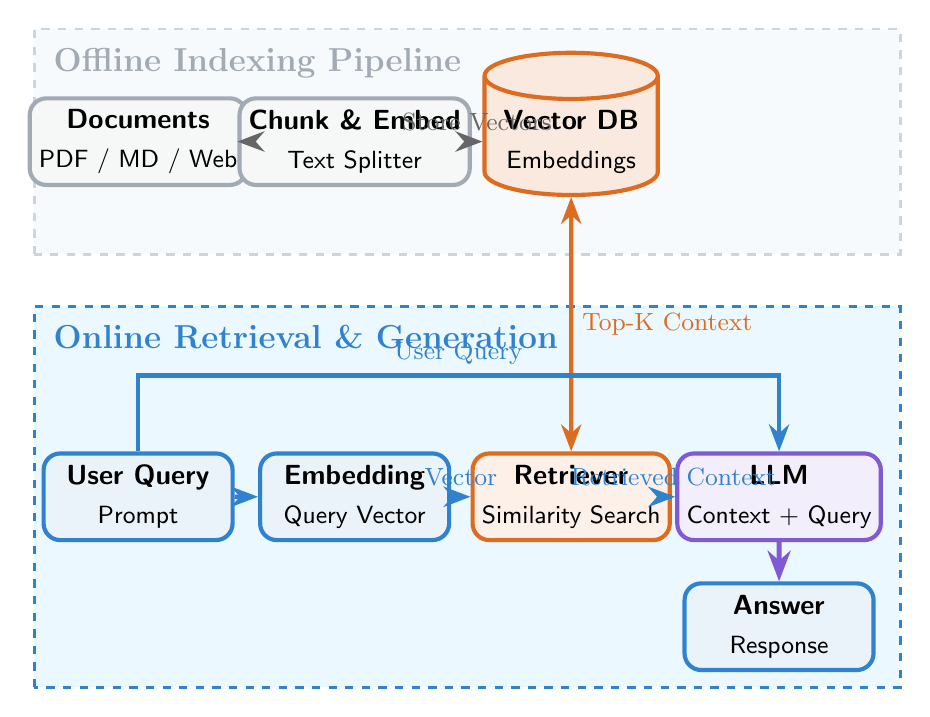
\begin{tikzpicture}[
    scale=1.1,
    >=Stealth,
    line width=1.2pt,
    font=\sffamily,
    block/.style={draw=#1, fill=#1!10, rounded corners=6pt, line width=1.5pt, minimum width=2.4cm, minimum height=1.1cm, align=center},
    cylinder_style/.style={draw=dbcolor, fill=dbcolor!15, shape=cylinder, aspect=0.3, cylinder uses custom fill, cylinder end fill=dbcolor!30, line width=1.5pt, minimum width=2.2cm, minimum height=1.6cm, align=center, shape border rotate=90}
]

    % Offline Indexing Pipeline Box (Top)
    \fill[offlinebg, draw=offlineborder, dashed, line width=1pt] (-5.0, 1.8) rectangle (5.0, 4.4);
    \node[offlineborder!80!black, font=\bfseries\large, anchor=north west] at (-4.9, 4.3) {Offline Indexing Pipeline};

    % Online Query Pipeline Box (Bottom)
    \fill[onlinebg, draw=onlineborder, dashed, line width=1pt] (-5.0, -3.2) rectangle (5.0, 1.2);
    \node[onlineborder, font=\bfseries\large, anchor=north west] at (-4.9, 1.1) {Online Retrieval \& Generation};

    % Offline Components
    \node[block=offlineborder!80!black] (docs) at (-3.8, 3.1) {\textbf{Documents}\\[2pt]\small PDF / MD / Web};
    \node[block=offlineborder!80!black] (chunk) at (-1.3, 3.1) {\textbf{Chunk \& Embed}\\[2pt]\small Text Splitter};

    % Shared Vector DB (Middle Right)
    \node[cylinder_style] (vdb) at (1.2, 3.1) {\textbf{Vector DB}\\[2pt]\small Embeddings};

    % Online Components
    \node[block=onlineborder] (user) at (-3.8, -1.0) {\textbf{User Query}\\[2pt]\small Prompt};
    \node[block=onlineborder] (qembed) at (-1.3, -1.0) {\textbf{Embedding}\\[2pt]\small Query Vector};
    \node[block=dbcolor] (retriever) at (1.2, -1.0) {\textbf{Retriever}\\[2pt]\small Similarity Search};
    \node[block=llmcolor] (llm) at (3.6, -1.0) {\textbf{LLM}\\[2pt]\small Context + Query};
    \node[block=onlineborder] (ans) at (3.6, -2.5) {\textbf{Answer}\\[2pt]\small Response};

    % Flow Arrows - Offline
    \draw[->, line width=1.5pt, gray!80!black] (docs) -- (chunk);
    \draw[->, line width=1.5pt, gray!80!black] (chunk) -- (vdb) node[midway, above, font=\small] {Store Vectors};

    % Flow Arrows - Online
    \draw[->, line width=1.5pt, onlineborder] (user) -- (qembed);
    \draw[->, line width=1.5pt, onlineborder] (qembed) -- (retriever) node[midway, above, font=\small] {Vector};

    % Retrieval connection from Vector DB
    \draw[<->, line width=1.5pt, dbcolor] (vdb) -- (retriever) node[midway, right, font=\small] {Top-K Context};

    % Context & Query to LLM
    \draw[->, line width=1.5pt, onlineborder] (retriever) -- (llm) node[midway, above, font=\small] {Retrieved Context};
    \draw[->, line width=1.5pt, onlineborder] (user) |- (-3.8, 0.4) -| (llm) node[near start, above, font=\small] {User Query};

    % LLM to Answer
    \draw[->, line width=1.8pt, llmcolor] (llm) -- (ans);

\end{tikzpicture}
\end{document}
